\chapter{Hilbert空间上的紧算子}\vspace{-2em}

对于有限维空间中的线性算子 $A : {\mathbb{R}}^{n} \mapsto  {\mathbb{R}}^{n}$ ，其核、值域、特征值与特征向量等方面已有若干结论.特别地:

(i) $A$ 是单射当且仅当 $A$ 是满射.事实上，子空间 $\operatorname{Ker}\left( A\right)$ 与 ${\left(  \operatorname{Range}\left( A\right) \right)  }^{ \bot  }$ 具有相同维数.

(ii) 若 $A$ 是对称的，则其特征值为实数；此外，空间 ${\mathbb{R}}^{n}$ 存在一组由 $A$ 的特征向量构成的标准正交基.

本章中，我们将证明类似结论，其适用于Hilbert空间 $H$ 上的无穷维算子 $\Lambda$ .事实上，(i) 对形如 $\Lambda  = I - K$ 的算子仍成立，其中 $I$ 是恒等算子， $K$ 是紧算子；此外，(ii) 中的命题可推广至任意紧自伴算子 $\Lambda  : H \mapsto  H$ .

\section{Fredholm理论}

设 $H$ 是一个Hilbert空间.我们回顾:有界线性算子 $K$ : $H \mapsto  H$ 是紧的，若对任意有界点列 ${u}_{n} \in  H$ ，均可提取子列 ${\left( {u}_{{n}_{j}}\right) }_{j \geq  1}$ ，使得像收敛: $K{u}_{{n}_{j}} \rightarrow  v$ (对某个 $v \in  H$ ).

下一个定理描述了形如 $I - K$ 的算子及其伴随算子的核与值域之间的若干关系.

\begin{theorem}[Fredholm]\label{thm:fredholm}
设 $H$ 是实数域上的Hilbert空间， $K : H \mapsto  H$ 是紧线性算子，则

(i) $\operatorname{Ker}\left( {I - K}\right)$ 是有限维的；

(ii) $\operatorname{Range}\left( {I - K}\right)$ 是闭的；

(iii) $\operatorname{Range}\left( {I - K}\right)  = \operatorname{Ker}{\left( I - {K}^{ * }\right) }^{ \bot  }$ ；

(iv) $\operatorname{Ker}\left( {I - K}\right)  = \{ 0\}$ 当且仅当 $\operatorname{Range}\left( {I - K}\right)  = H$ ；

(v) $\operatorname{Ker}\left( {I - K}\right)$ 与 $\operatorname{Ker}\left( {I - {K}^{ * }}\right)$ 具有相同维数.
\end{theorem}

\begin{proof}
1. 若 $\left( {I - K}\right)$ 的核是无穷维的，则可在 $\operatorname{Ker}\left( {I - K}\right)$ 中找到一列标准正交序列 ${\left( {e}_{n}\right) }_{n \geq  1}$ .此时对每个 $n$ 有 $K{e}_{n} = {e}_{n}$ ；此外，由勾股定理，对 $m \neq  n$ 有
\[
\norm{e_m-e_n}^{2} = \norm{e_m}^{2} + \norm{e_n}^{2} = 2
\]

因此对每个 $m \neq  n$ 有 $\norm{K{e}_{m} - K{e}_{n}} = \norm{{e}_{m} - {e}_{n}} = \sqrt{2}$ .故从序列 ${\left( K{e}_{n}\right) }_{n \geq  1}$ 中无法提取任何收敛子列.这一矛盾确立了 (i).

\noindent 2. 为证 (ii)，我们首先证明存在 $\beta  > 0$ ，使得
\begin{equation}\tag{6.1}\label{eq:fredholm-estimate}
\| u - {Ku}\|  \geq  \beta \| u\|,\;\forall\,u \in  \operatorname{Ker}{\left( I - K\right) }^{ \bot  }.
\end{equation}

事实上，若\eqref{eq:fredholm-estimate}不成立，则可找到点列 ${u}_{n} \in  \operatorname{Ker}{\left( I - K\right) }^{ \bot  }$ ，使得 $\norm{u}_{n} = 1$ 且 $\norm{{u}_{n} - K{u}_{n}} < 1/n$ .

由于序列 ${\left( {u}_{n}\right) }_{n \geq  1}$ 有界，通过提取子列并重新标号，可设该序列弱收敛，即 ${u}_{n} \rightharpoonup  u$ (对某个 $u \in  H$ ).

由于 $K$ 是紧算子，由定理\ref{thm:compact-weak-to-strong}可知这蕴含强收敛 $K{u}_{n} \rightarrow  {Ku}$ .我们现得到
\[
\norm{{u}_{n} - {Ku}}\; \leq  \;\norm{{u}_{n} - K{u}_{n}} + \norm{K{u}_{n} - {Ku}}\; \rightarrow  ,\;0\;\text{ 当 }\,n \rightarrow  \infty .
\]
这给出强收敛 ${u}_{n} \rightarrow  {Ku}$ .结合弱收敛 ${u}_{n} \rightharpoonup  u$ ，可知 $u = {Ku}$ 与 ${u}_{n} \rightarrow  u$ 均强收敛.

由构造可知，我们现已有
\[
\| u\|  = \mathop{\lim }\limits_{{n \rightarrow  \infty }}\norm{u}_{n} = 1,\;u \in  \operatorname{Ker}{\left( I - K\right) }^{ \bot  },
\]

但同时， $u - {Ku} = 0$ ，故 $u \in  \operatorname{Ker}\left( {I - K}\right)$ .因此我们得出矛盾，从而证得\eqref{eq:fredholm-estimate}.

\noindent 3. 我们现证明 Range $\left( {I - K}\right)$ 是闭的.考虑点列 ${v}_{n} \in  \operatorname{Range}\left( {I - K}\right)$ ，其中 ${v}_{n} \rightarrow  v$ 当 $n \rightarrow  \infty$ .我们需要找到某个 $u$ ，使得 $v = u - {Ku}$ .由假设，对每个 $n \geq  1$ ，存在 ${u}_{n}$ 满足 ${v}_{n} = {u}_{n} - K{u}_{n}$ .注意，若对某个 $u \in  H$ 有 ${u}_{n} \rightarrow  u$ ，则由连续性可立即推出 $v = u - {Ku}$ .但一般而言，无法保证序列 ${\left( {u}_{n}\right) }_{n \geq  1}$ 收敛.

为克服这一困难，令 ${\widetilde{u}}_{n}$ 为 ${u}_{n}$ 在 $\operatorname{Ker}\left( {I - K}\right)$ 上的正交投影，并令 ${z}_{n} \doteq  {u}_{n} - {\widetilde{u}}_{n}$.这些定义导出
\[
{z}_{n}\; \doteq  \;{u}_{n} - {\widetilde{u}}_{n}\; \in  \mathrm{{Ker}}{\left( I - K\right) }^{ \bot  },\;{v}_{n}\; = \;{u}_{n} - K{u}_{n}\; = \;{z}_{n} - K{z}_{n}\;.
\]

利用\eqref{eq:fredholm-estimate}，对任意指标对 $m,n$ ，我们得到
\[
\norm{{v}_{m} - {v}_{n}} \geq  \beta \norm{{z}_{m} - {z}_{n}}.
\]

由于序列 ${\left( {v}_{n}\right) }_{n \geq  1}$ 是 Cauchy 列，这表明序列 ${\left( {z}_{n}\right) }_{n \geq  1}$ 也是 Cauchy 列.因此存在 $u \in  H$ ，使得 ${z}_{n} \rightarrow  u$ ，从而有
\[
u - {Ku} = \mathop{\lim }\limits_{{n \rightarrow  \infty }}{z}_{n} - K{z}_{n} = \mathop{\lim }\limits_{{n \rightarrow  \infty }}{v}_{n} = v
\]

\begin{figure}[htbp]
\centering
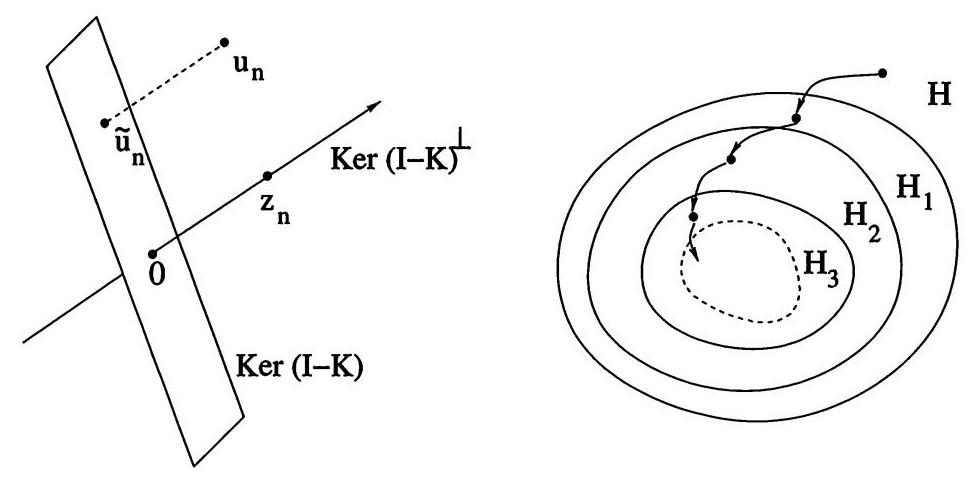
\includegraphics[width=0.9\textwidth]{images/bo_d6ik6nn7aajc739ct1l0_115_253_988_972_477_0.jpg}
\caption{左:通过选取 ${z}_{n} \in  \operatorname{Ker}{\left( I - K\right) }^{ \bot  }$ ，我们实现不等式 $\beta \norm{z}_{n} \leq  \norm{v}_{n}$ ，该式在 (ii) 的证明中使用.右:若 $I - K$ 是单射但不满射，则子空间列 ${H}_{n} \doteq \; {\left( I - K\right) }^{n}\left( H\right)$ 严格递减.这导致矛盾，用于 (iv) 的证明.}
\label{fig:fredholm-proof-geometry}
\end{figure}

\noindent 4. 由于 Range $\left( {I - K}\right)$ 与 $\operatorname{Ker}{\left( I - {K}^{ * }\right) }^{ \bot  }$ 均为闭子空间，断言 (iii) 成立当且仅当
\begin{equation}\tag{6.2}\label{eq:fredholm-range-orth-ker-adjoint}
\operatorname{Range}{\left( I - K\right) }^{ \bot  } = \operatorname{Ker}\left( {I - {K}^{ * }}\right) .
\end{equation}

这可通过观察以下命题彼此等价而得证:
{\setjot[-3]\begin{align*}
    x &\in  \operatorname{Ker}\left( {I - {K}^{ * }}\right) , \\
    \left( {I - {K}^{ * }}\right) x &= 0, \\
    \left( {y,\left( {I - {K}^{ * }}\right) x}\right)  &= 0,\;\forall\,\;y \in  H, \\
    \left( {\left( {I - K}\right) y,x}\right)  &= 0,\;\forall\,\;y \in  H, \\
    x &\in  \operatorname{Range}{\left( I - K\right) }^{ \bot  }.
\end{align*}}


\noindent 5. 为证明 (iv)，假设 $\operatorname{Ker}\left( {I - K}\right)  = \{ 0\}$ ，即算子 $I - K$ 是单射.若 $\operatorname{Range}\left( {I - K}\right)  \neq  H$，我们将导出矛盾.

事实上，假设该值域并非整个空间: ${H}_{1} \doteq  (I - \; K)\left( H\right)  \neq  H$ .由(ii)可知， ${H}_{1}$ 是 $H$ 的一个闭子空间.由于 $I - K$ 是单射，必有
\[
{H}_{2} \doteq  \left( {I - K}\right) \left( {H}_{1}\right)  \subset  {H}_{1}.
\]

我们可通过归纳法继续此过程:对每个 $n$ ，定义
\[
{H}_{n} \doteq  {\left( I - K\right) }^{n}\left( H\right) .
\]

由归纳法可知，每个 ${H}_{n}$ 均为 $H$ 的闭子空间，且
\[
H \supset  {H}_{1} \supset  {H}_{2} \supset  \cdots
\]

对每个 $n \geq  1$ ，现取向量 ${e}_{n} \in  {H}_{n} \cap  {H}_{n + 1}^{ \bot  }$ 使得 $\norm{e}_{n} = 1$ .注意，若 $m < n$ ，则
\[
K{e}_{m} - K{e}_{n} =  - \left( {{e}_{m} - K{e}_{m}}\right)  + \left( {{e}_{n} - K{e}_{n}}\right)  + \left( {{e}_{m} - {e}_{n}}\right)  = {e}_{m} + {z}_{m}
\]

其中 ${z}_{m} \doteq   - \left( {{e}_{m} - K{e}_{m}}\right)  + \left( {{e}_{n} - K{e}_{n}}\right)  - {e}_{n} \in  {H}_{m + 1}$ .

由于 ${e}_{m} \in  {H}_{m + 1}^{ \bot  }$ ，由勾股定理可知
\[
\norm{K{e}_{m} - K{e}_{n}} \geq  \norm{e}_{m} = 1
\]

因此，序列 ${\left( K{e}_{n}\right) }_{n \geq  1}$ 不可能有任何强收敛子列，与 $K$ 的紧性矛盾.

\noindent 6. 为证明(iv)的逆命题，我们采用对偶性论证.假设 $\operatorname{Range}\left( {I - K}\right)  = H$ .由定理\ref{thm:adjoint-properties}，
\[
\operatorname{Ker}\left( {I - {K}^{ * }}\right)  = \operatorname{Range}{\left( I - K\right) }^{ \bot  } = {H}^{ \bot  } = \{ 0\} .
\]
由于 ${K}^{ * }$ 是紧算子，由前一步可知 $\operatorname{Range}\left( {I - {K}^{ * }}\right)  = H$ .再次应用定理\ref{thm:adjoint-properties}，即得 $\operatorname{Ker}\left( {I - K}\right)  = \operatorname{Range}{\left( I - {K}^{ * }\right) }^{ \bot  } = {H}^{ \bot  } = \{ 0\}$ ，结论成立.

\noindent 7. 为证明(v)，我们首先说明 $\operatorname{Ker}\left( {I - K}\right)$ 的维数不小于 Range ${\left( I - K\right) }^{ \bot  }$ 的维数.事实上，反设
\begin{equation}\tag{6.3}\label{eq:fredholm-dim-inequality}
\dim \operatorname{Ker}\left( {I - K}\right)  < \dim \operatorname{Range}{\left( I - K\right) }^{ \bot  }.
\end{equation}

则存在一个线性映射 $A : \operatorname{Ker}\left( {I - K}\right)  \mapsto  \operatorname{Range}{\left( I - K\right) }^{ \bot  }$ ，其为单射但非满射.我们将 $A$ 扩展为定义在整个空间 $H$ 上的线性映射 $A : H \mapsto$ :Range ${\left( I - K\right) }^{ \bot  }$ ，要求当 $u \in  \operatorname{Ker}{\left( I - K\right) }^{ \bot  }$ 时 ${Au} = 0$ .由于 $A$ 的值域是有限维的，故算子 $A$ 是紧的，从而 $K + A$ 也是紧的.

我们声称 $\operatorname{Ker}\left( {I - \left( {K + A}\right) }\right)  = \{ 0\}$ .事实上，任取向量 $u \in  H$ 并将其写为
\[
u = {u}_{1} + {u}_{2},\;{u}_{1} \in  \operatorname{Ker}\left( {I - K}\right) ,\;{u}_{2} \in  \operatorname{Ker}{\left( I - K\right) }^{ \bot  }.
\]

由此得到
\begin{equation}\tag{6.4}\label{eq:fredholm-direct-sum-decomposition}
\left( {I - K - A}\right) \left( {{u}_{1} + {u}_{2}}\right) 
= \left( {I - K}\right) {u}_{2} - A{u}_{1}
\in  \operatorname{Range}\left( {I - K}\right)  \oplus  \operatorname{Range}{\left( I - K\right) }^{ \bot  }.
\end{equation}

由于 $\left( {I - K}\right) {u}_{2}$ 与 $A{u}_{1}$ 正交，和式 $\left( {I - K}\right) {u}_{2} + A{u}_{1}$ 仅当 $\left( {I - K}\right) {u}_{2} = 0$ 且 $A{u}_{1} = 0$ 时才能为零.回顾算子 $I - K$ 在 $\operatorname{Ker}{\left( I - K\right) }^{ \bot  }$ 上是一对一的，且 $A$ 在 $\operatorname{Ker}\left( {I - K}\right)$ 上是一对一的，我们得出 ${u}_{1} = {u}_{2} = 0$ .

将(iv)应用于紧算子 $K + A$ ，得到值域 $(I - \; \left( {K + A}\right) ) = H$ .然而这是不可能的:由构造可知，存在一个向量 $v \in  \operatorname{Range}{\left( I - K\right) }^{ \bot  }$ 满足 $v \notin  \operatorname{Range}\left( A\right)$ .根据\eqref{eq:fredholm-direct-sum-decomposition}，方程
\[
u - {Ku} - {Au} = v
\]

无解.这一矛盾表明\eqref{eq:fredholm-dim-inequality}不可能成立.

\noindent 8. 回顾值域 ${\left( I - {K}^{ * }\right) }^{ \bot  } = \operatorname{Ker}\left( {I - K}\right)$ ，由前一步可推出
\[
\dim \operatorname{Ker}\left( {I - {K}^{ * }}\right)  \geq  \dim \operatorname{Range}{\left( I - {K}^{ * }\right) }^{ \bot  } = \dim \operatorname{Ker}\left( {I - K}\right) .
\]

交换 $K$ 与 ${K}^{ * }$ 的角色，可得相反的不等式.
\end{proof}

\begin{note}[Fredholm择一性]\label{rem:fredholm-alternative}
当 $K$ 为紧算子时，上述定理提供了关于线性方程
\begin{equation}\tag{6.5}\label{eq:fredholm-equation}
u - {Ku} = f.
\end{equation}

解的存在性与唯一性的信息.具体而言，可能出现两种情形.

情形1: $\operatorname{Ker}\left( {I - K}\right)  = \{ 0\}$ .此时算子 $I - K$ 是一对一且满射的.对任意 $f \in  H$ ，方程\eqref{eq:fredholm-equation}恰有唯一解.

情形2: $\operatorname{Ker}\left( {I - K}\right)  \neq  \{ 0\}$ .这意味着齐次方程 $u - {Ku} = 0$ 具有非平凡解.此时，方程\eqref{eq:fredholm-equation}有解当且仅当 $f \in  \operatorname{Ker}{\left( I - {K}^{ * }\right) }^{ \bot  }$ ，即当且仅当
\begin{equation}\tag{6.6}\label{eq:fredholm-solvability-condition}
\left( {f,u}\right)  = 0,\;\forall\,u \in  H,\st u - {K}^{ * }u = 0.
\end{equation}

上述二分法称为Fredholm择一性.
\end{note}

\section{紧算子的谱}

设 $H$ 为实数域上的Hilbert空间， $\Lambda  : H \mapsto  H$ 为有界线性算子.
\begin{definition}[预解集、谱]
    $\Lambda$ 的\colorbf{预解集}是满足 ${\eta I} - \Lambda$ 为双射的所有数 $\eta  \in  \mathbb{R}$ 构成的集合，记作\colorbf{$\rho \left( \Lambda \right)$}.\par
    称预解集的补集为 $\Lambda$ 的\colorbf{谱}，记作\colorbf{$\sigma \left( \Lambda \right)  \doteq  \mathbb{R} \setminus  \rho \left( \Lambda \right)$}.
\end{definition}
注意，在此情形下，由开映射定理，逆算子 ${\left( \eta I - \Lambda \right) }^{-1}$ 是连续的.
\begin{definition}[点谱]
    $\Lambda$ 的\colorbf{点谱}是使 ${\eta I} - \Lambda$ 不是一对一的所有数 $\eta  \in  \mathbb{R}$ 构成的集合，记作\colorbf{${\sigma }_{p}\left( \Lambda \right)$}.等价地， $\eta  \in  {\sigma }_{p}\left( \Lambda \right)$ 当且仅当存在非零向量 $w \in  H$ 使得\[
{\Lambda w} = {\eta w}
\]
此时， $\eta$ 称为 $\Lambda$ 的一个\colorbf{特征值}， $w$ 为其对应的\colorbf{特征向量}.\par
\end{definition}

\begin{definition}[本质谱]
    $\Lambda$ 的\colorbf{本质谱}是满足 ${\eta I} - \Lambda$ 是单射但不是满射的所有数 $\eta  \in  \mathbb{R}$ 构成的集合，记作\colorbf{${\sigma }_{e}\left( \Lambda \right)  = \sigma \left( \Lambda \right)  \setminus  {\sigma }_{p}\left( \Lambda \right)$}.
\end{definition}





\begin{theorem}[紧算子的谱]\label{thm:compact-operator-spectrum}
设 $H$ 是一个无限维Hilbert空间， $K : H \mapsto  H$ 是一个紧线性算子.则
\begin{enumerate}[(i)]
    \item $0 \in  \sigma \left( K\right)$ .
    \item $\sigma \left( K\right)  = {\sigma }_{p}\left( K\right)  \cup  \{ 0\}$ .
    \item 要么 ${\sigma }_{p}\left( K\right)$ 是有限集，要么 ${\sigma }_{p}\left( K\right)  = \left\{  {{\lambda }_{k};k \geq  1}\right\}$，其中特征值满足 $\mathop{\lim }\limits_{{k \rightarrow  \infty }}{\lambda }_{k} = 0$.
\end{enumerate}
\end{theorem}

\begin{proof}
1. 为证 (i)，采用反证法.若 $0 \notin  \sigma \left( K\right)$ ，则 $K$ 存在连续逆算子 ${K}^{-1} : H \mapsto  H$ .于是有 $I = K \circ  {K}^{-1}$ .由于连续算子与紧算子的复合仍是紧算子，这将推出恒等算子是紧算子.但这不成立，因为 $H$ 是无限维空间，且 $H$ 中的闭单位球非紧.

\noindent 2. 为证 (ii)，假设 $\lambda  \in  \sigma \left( K\right)$ ，其中 $\lambda  \neq  0$ .若 $\operatorname{Ker}\left( {{\lambda I} - K}\right)  = \{ 0\}$ ，Fredholm择一性将推出 $\operatorname{Range}\left( {{\lambda I} - K}\right)  = H$ .再由开映射定理， $\left( {{\lambda I} - K}\right)$ 将具有有界逆，与假设矛盾.该矛盾表明 $\lambda  \in  {\sigma }_{p}\left( K\right)$ .

\noindent 3. 为证 (iii)，假设 ${\left( {\lambda }_{n}\right) }_{n \geq  1}$ 是 $K$ 的一列互异特征值，且满足 ${\lambda }_{n} \rightarrow  \lambda$ .我们声称 $\lambda  = 0$.

事实上，由于 ${\lambda }_{n} \in  {\sigma }_{p}\left( K\right)$ ，对每个 $n \geq  1$ ，存在特征向量 ${w}_{n}$ 使得 $K{w}_{n} = {\lambda }_{n}{w}_{n}$.记 ${H}_{n} \doteq  \operatorname{span}\left\{  {{w}_{1},\ldots ,{w}_{n}}\right\}$ .因对应于互异特征值的特征向量线性无关，故 ${H}_{n} \subset  {H}_{n + 1}$.

注意，对任意 $n \geq  2$ ，均有 $\left( {K - {\lambda }_{n}I}\right) {H}_{n} \subseteq  {H}_{n - 1}$ .因此对每个 $n$ ，可选取元素 ${e}_{n} \in  {H}_{n} \cap  {H}_{n - 1}^{ \bot  }$ 使得 $\norm{e}_{n} = 1$ .若 $m < n$ ，则
\[
\left( {K{e}_{n} - {\lambda }_{n}{e}_{n}}\right)  \in  {H}_{n - 1}\;,\;\left( {K{e}_{m} - {\lambda }_{m}{e}_{m}}\right)  \in  {H}_{m - 1} \subset  {H}_{n - 1}\;,
\]

且 ${e}_{m} \in  {H}_{m} \subseteq  {H}_{n - 1}$ ，而 ${e}_{n} \in  {H}_{n - 1}^{ \bot  }$ .故
{\setjot[-2]\begin{align*}
\norm{K{e}_{n} - K{e}_{m}} &= \norm{\left( {K{e}_{n} - {\lambda }_{n}{e}_{n}}\right)  - \left( {K{e}_{m} - {\lambda }_{m}{e}_{m}}\right)  + {\lambda }_{n}{e}_{n} - {\lambda }_{m}{e}_{m}}\\
&\geq  \norm{{\lambda }_{n}{e}_{n}} = \left| {\lambda }_{n}\right| .
\end{align*}}

因此
\[
\mathop{\liminf }\limits_{{m,n \rightarrow  \infty }}\norm{K{e}_{n} - K{e}_{m}} \geq  \mathop{\lim }\limits_{{n \rightarrow  \infty }}\left| {\lambda }_{n}\right|  = \left| \lambda \right|
\]

若 $\left| \lambda \right|  > 0$ ，则序列 ${\left( K{e}_{n}\right) }_{n \geq  1}$不能有任何收敛子列，与 $K$ 是紧集的假设矛盾.
\end{proof}

\section{自伴算子}
\begin{definition}[对称算子]
    
设 $\Lambda  : H \mapsto  H$ 为实Hilbert空间 $H$ 上的有界线性算子.若 $\Lambda$ 满足
\[
\left( {\Lambda \bm{x},\bm{y}}\right)  = \left( {\bm{x},\Lambda \bm{y}}\right) \;\forall\,\bm{x},\bm{y} \in  H.
\]
则称 $\Lambda$ 是\colorbf{对称的}.
\end{definition}

注意，这等价于说 $\Lambda$ 是自伴的.

\begin{instance}\label{ins:symmetric-matrix-extremal-eigenvalues}
设 $A = {\left( {a}_{ij}\right) }_{i,j = 1,\ldots ,n}$ 是一个对称的 $n \times  n$ 矩阵，则 $A$ 确定了一个从 ${\mathbb{R}}^{n}$ 到 ${\mathbb{R}}^{n}$ 的对称线性算子 $\bm{x} \mapsto  A\bm{x}$ .它还确定了二次型
\[
\bm{x} \mapsto  \langle \bm{x},A\bm{x}\rangle  = \mathop{\sum }\limits_{{i,j = 1}}^{n}{a}_{ij}{x}_{i}{x}_{j}.
\]

下列量
\[
m \doteq  \mathop{\min }\limits_{{\left| \bm{x}\right|  = 1}}\langle \bm{x},A\bm{x}\rangle ,\;M \doteq  \mathop{\max }\limits_{{\left| \bm{x}\right|  = 1}}\langle \bm{x},A\bm{x}\rangle
\]

分别给出 $A$ 的最小与最大特征值.
\end{instance}

Hilbert空间上对称线性算子的理论，将对称矩阵的诸多熟知性质推广至无穷维情形.

\begin{lemma}[对称算子谱的界]\label{lem:selfadjoint-spectrum-bounds}
设 $\Lambda  : H \mapsto  H$ 是实Hilbert空间 $H$ 上的有界线性自伴算子.定义上下界
\[
m \doteq  \mathop{\inf }\limits_{{u \in  H,\| u\|  = 1}}\left( {{\Lambda u},u}\right) ,\;M \doteq  \mathop{\sup }\limits_{{u \in  H,\| u\|  = 1}}\left( {{\Lambda u},u}\right) .
\]
则
\begin{enumerate}
    \item 谱 $\sigma \left( \Lambda \right)$ 包含于区间 $\left(  {m,M}\right)$ 中.
    \item $m,M \in  \sigma \left( \Lambda \right)$ .
    \item $\| \Lambda \|  = \max \{  - m,M\}$ .
\end{enumerate}
\end{lemma}

\begin{proof}
1. 设 $\eta  > M$ .则
\[
\left( {{\eta u} - {\Lambda u},u}\right)  \geq  \left( {\eta  - M}\right) \| u{\| }^{2}\;\forall\,u \in  H.
\]

由定理\ref{thm:lax-milgram}，线性连续算子 ${\eta I} - \Lambda$ 是单射且满射.由开映射定理，它具有连续逆.这表明每个 $\eta  > M$ 均属于 $\Lambda$ 的预解集.类似地，将 $\Lambda$ 替换为 $- \Lambda$ ，可知每个 $\eta  < m$ 亦属于预解集.这就证明了(i).

\noindent 2. 此后，为明确起见，我们假设 $\left| m\right|  \leq  M$ .相反情形(即 $M <  - m$ )可用完全类似的论证处理，只需将 $\Lambda$ 替换为 $- \Lambda$ 即可.

对每个 $u,v \in  H$ ，有
{\setjot[-2]\begin{align*}
    4\left( {{\Lambda u},v}\right)  &= \left( {\Lambda \left( {u + v}\right) ,u + v}\right)  - \left( {\Lambda \left( {u - v}\right) ,u - v}\right)\\
    &\leq  M\left( {\| u + v{\| }^{2} + \| u - v{\| }^{2}}\right)\\
    &= {2M}\left( {\| u{\| }^{2} + \| v{\| }^{2}}\right) .
\end{align*}}

若 ${\Lambda u} \neq  0$ ，令 $v \doteq  \left( {\| u\| /\| {\Lambda u}\| }\right) {\Lambda u}$ ，则得
\[
2\| u\| \| {\Lambda u}\|  = 2\left( {{\Lambda u},v}\right)  \leq  M\left( {\| u{\| }^{2} + \| v{\| }^{2}}\right)  = {2M}\| u{\| }^{2}.
\]

因此
\begin{equation}\tag{6.7}\label{eq:selfadjoint-operator-bound}
\| {\Lambda u}\|  \leq  M\| u\| \;\forall\,u \in  H.
\end{equation}

事实上，\eqref{eq:selfadjoint-operator-bound} 在 ${\Lambda u} = 0$ 时亦平凡成立.

由于 $\| \Lambda \|  \geq  \mathop{\sup }\limits_{{\| u\|  = 1}}\left( {{\Lambda u},u}\right)  = M$ ，由\eqref{eq:selfadjoint-operator-bound}可得 $\| \Lambda \|  = M$ ，从而证明(iii).

\noindent 3. 接下来，我们断言 $M \in  \sigma \left( \Lambda \right)$ .取一序列 ${\left( {u}_{n}\right) }_{n \geq  1}$ ，满足
\[
\left( {\Lambda {u}_{n},{u}_{n}}\right)  \rightarrow  M,\;\norm{u}_{n} = 1\;\forall\,n.
\]

则
{\setjot[-2]\begin{align*}
    \norm{\Lambda {u}_{n} - Mu_n}^{2} &= {\norm{\Lambda u_n}}^{2} - {2M}\left( {\Lambda {u}_{n},{u}_{n}}\right)  + {M}^{2}{\norm{u_n}}^{2} \\
    &\leq  2{M}^{2} - {2M}\left( {\Lambda {u}_{n},{u}_{n}}\right)  \rightarrow  0.
\end{align*}}

因此算子 $\Lambda  - {MI}$ 不可能具有有界逆.
\end{proof}

根据线性代数中一个经典定理，每个对称的 $n \times  n$ 矩阵 $A$ 均可通过正交变换化为对角形式.这可通过选取由 ${\mathbb{R}}^{n}$ 的特征向量构成的标准正交基来实现.以下定理表明，该结论对紧对称算子依然成立.

\begin{theorem}[Hilbert--Schmidt；紧对称算子的特征向量]\label{thm:hilbert-schmidt}
设 $H$ 为可分实Hilbert空间， $K : H \mapsto  H$ 为紧对称线性算子.则存在由 $K$ 的特征向量构成的 $H$ 的可数标准正交基.
\end{theorem}

\begin{proof}
1. 若 $H = {\mathbb{R}}^{n}$ ，此为线性代数中的经典结论.因此我们假设 $H$ 是无限维的.令 ${\eta }_{0} = 0$ ，并令 $\left\{  {{\eta }_{1},{\eta }_{2},\ldots }\right\}$ 表示 $K$ 的所有非零特征值之集.考虑特征子空间
\[
{H}_{0} \doteq  \operatorname{Ker}\left( K\right) ,{H}_{1} \doteq  \operatorname{Ker}\left( {K - {\eta }_{1}I}\right) ,{H}_{2} \doteq  \operatorname{Ker}\left( {K - {\eta }_{2}I}\right) ,\ldots .
\]

注意 $0 \leq  \dim \left( {H}_{0}\right)  \leq  \infty$ ，而对每个 $k \geq  1$ ，均有 $0 < \dim \left( {H}_{k}\right)  < \infty$ .

\noindent 2. 我们断言，若$m \neq  n$，子空间 ${H}_{m}$ 与 ${H}_{n}$ 正交.事实上，设 $u \in  {H}_{m},v \in  {H}_{n}$ ，则
\[
{\eta }_{m}\left( {u,v}\right)  = \left( {{Ku},v}\right)  = \left( {u,{Kv}}\right)  = {\eta }_{n}\left( {u,v}\right) .
\]

由于 ${\eta }_{m} \neq  {\eta }_{n}$ ，这推出 $\left( {u,v}\right)  = 0$ .

\noindent 3. 接下来，我们证明子空间 ${H}_{k}$ 生成整个空间 $H$ .更准确地说，考虑所有线性组合构成的集合
\[
\widetilde{H} \doteq  \left\{  {\mathop{\sum }\limits_{{k = 1}}^{N}{\alpha }_{k}{u}_{k};N \geq  1,{u}_{k} \in  {H}_{k},{\alpha }_{k} \in  \mathbb{R}}\right\}  .
\]

我们断言
\begin{equation}\tag{6.8}\label{eq:hilbert-schmidt-orthogonal-complement}
{\widetilde{H}}^{ \bot  } \subseteq  \operatorname{Ker}\left( K\right)  \doteq  {H}_{0}.
\end{equation}

事实上， $K\left( \widetilde{H}\right)  \subseteq  \widetilde{H}$ .\par
此外，若 $u \in  {\widetilde{H}}^{ \bot  }$ 且 $v \in  \widetilde{H}$ ，则 ${Kv} \in  \widetilde{H}$ ，从而有
\[
\left( {{Ku},v}\right)  = \left( {u,{Kv}}\right)  = 0.
\]
这表明 $K\left( {\widetilde{H}}^{ \bot  }\right)  \subseteq  {\widetilde{H}}^{ \bot  }$ .

令 $\widetilde{K}$ 为 $K$ 在子空间 ${\widetilde{H}}^{ \bot  }$ 上的限制.显然， $\widetilde{K}$ 是紧致、对称的算子.由引理\ref{lem:selfadjoint-spectrum-bounds}可知
\[
\| \widetilde{K}\|  = \mathop{\sup }\limits_{{u \in  {\widetilde{H}}^{ \bot  },\| u\|  = 1}}\left| \left( {\widetilde{K}u,u}\right) \right|  \doteq  M.
\]

若 $M \neq  0$ ，则由引理\ref{lem:selfadjoint-spectrum-bounds}可知， $\lambda  = M$ 或 $\lambda  =  - M$ 中至少一个属于 $\widetilde{K}$ 的谱.此时，由于 $\widetilde{K}$ 是紧算子， $\lambda$ 属于点谱，故存在特征向量 $w \in  {\widetilde{H}}^{ \bot  }$ 满足
\[
\widetilde{K}w = {Kw} = {\lambda w}.
\]

但这是不可能的，因为 $K$ 对应非零特征值的所有特征向量均已包含在子空间 ${H}_{k}$ 与 $k \geq  1$ 的并集中.因此我们得出 $\| \widetilde{K}\|  = 0$ ，从而证得\eqref{eq:hilbert-schmidt-orthogonal-complement}.

反过来，\eqref{eq:hilbert-schmidt-orthogonal-complement} 推出
\[
{\widetilde{H}}^{ \bot  } \subseteq  {H}_{0}^{ \bot  } \cap  {H}_{0} = \{ 0\} ,
\]

由此证明 $\widetilde{H}$ 在 $H$ 中稠密.

\noindent 4. 对每个 $k \geq  1$ ，有限维子空间 ${H}_{k}$ 存在标准正交基 ${\mathcal{B}}_{k} = \left\{  {{e}_{k,1},{e}_{k,2},\ldots ,{e}_{k,N\left( k\right) }}\right\}$ .此外，由于 $H$ 是可分的，其闭子空间 ${H}_{0} = \operatorname{Ker}\left( K\right)$ 存在可数标准正交基 ${\mathcal{B}}_{0} = \left\{  {{e}_{0,1},{e}_{0,2},\ldots }\right\}$ .因此，并集 $\mathcal{B} \doteq  \mathop{\bigcup }\limits_{{k \geq  0}}{\mathcal{B}}_{k}$ 构成 $H$ 的一个标准正交基.
\end{proof}

\begin{remark}\label{rem:compact-selfadjoint-solution-expansion}
设 $\left\{  {{\bm{w}}_{1},{\bm{w}}_{2},\ldots }\right\}$ 是实Hilbert空间 $H$ 的一个标准正交基，且均由线性、紧致、自伴算子 $K$ 的特征向量组成.令 ${\lambda }_{1},{\lambda }_{2},\ldots$ 为其对应的特征值.对给定的 $f \in  H$ ，考虑方程
\begin{equation}\tag{6.9}\label{eq:compact-selfadjoint-resolvent-equation}
u - {Ku} = f.
\end{equation}

若 $1 \notin  \sigma \left( K\right)$ ，则\eqref{eq:compact-selfadjoint-resolvent-equation}存在唯一解.记
\[
u = \mathop{\sum }\limits_{{k = 1}}^{\infty }{c}_{k}{\bm{w}}_{k},\;f = \mathop{\sum }\limits_{{k = 1}}^{\infty }{b}_{k}{\bm{w}}_{k},
\]

该解可计算为
\begin{equation}\tag{6.10}\label{eq:compact-selfadjoint-resolvent-series}
u = \mathop{\sum }\limits_{{k = 1}}^{\infty }\frac{{b}_{k}}{1 - {\lambda }_{k}}{\bm{w}}_{k} = \mathop{\sum }\limits_{{k = 1}}^{\infty }\frac{\left( f,{\bm{w}}_{k}\right) }{1 - {\lambda }_{k}}{\bm{w}}_{k}.
\end{equation}
\end{remark}

\begin{remark}\label{rem:density-span-criteria}
设 $S = \left\{  {{u}_{1},{u}_{2},\ldots }\right\}$ 是实数域上的 Banach 空间 $X$ 中的一个可数集，一个基本问题是判定 $\operatorname{span}\left( S\right)$ 在 $X$ 中是否稠密.在两种重要情形下可给出肯定回答.

(I) $X = \mathcal{C}\left( E\right)$ 是紧度量空间 $E$ 上所有连续实值函数构成的空间.此时，若 $\operatorname{span}\left( S\right)$ 是一个包含常值函数且能分离点的代数，则 Stone-Weierstrass 定理给出 $\overline{\operatorname{span}\left( S\right) } = X$.

(II) $X$ 是一个可分 Hilbert 空间，且存在一个紧自伴算子 $\Lambda  : X \mapsto  X$ ，使得

(i) $\operatorname{span}\left( S\right)$ 包含 $\Lambda$ 的所有特征向量，且

(ii) $\operatorname{span}\left( S\right)$ 包含 $\Lambda$ 的核.

此时，Hilbert-Schmidt 定理给出 $\overline{\operatorname{span}\left( S\right) } = X$ .
\end{remark}

\section{习题}

\begin{rbhw}[index=1]
(i) 求两个从 ${L}^{2}\left( \left(  {0,\infty }\right)  \right)$ 到自身的有界线性算子 ${\Lambda }_{1},{\Lambda }_{2}$ ，使得 ${\Lambda }_{1} \circ  {\Lambda }_{2} = I$ (恒等算子)，但 ${\Lambda }_{2} \circ  {\Lambda }_{1} \neq  I$ .

(ii) 设 $H$ 是一个实 Hilbert 空间， $\Lambda ,K : H \mapsto  H$ 是有界线性算子，且 $K$ 是紧算子.证明此时
\[
\Lambda \left( {I - K}\right)  = I\;\text{ if and only if }\;\left( {I - K}\right) \Lambda  = I.
\]
\end{rbhw}

\begin{rbhw}
在 Hilbert 空间 ${L}^{2}\left( \left(  {0,\infty }\right)  \right)$ 上，考虑由下式定义的线性算子:
\[
\left( {\Lambda f}\right) \left( x\right)  = {2f}\left( {x + 1}\right) ,\;x \geq  0.
\]

(i) $\Lambda$ 是否为有界算子？是否为紧算子？

(ii) 显式求出伴随算子 ${\Lambda }^{ * }$ .

(iii) 描述 $\operatorname{Ker}\left( \Lambda \right)$ 和 $\operatorname{Ker}\left( {\Lambda }^{ * }\right)$ .
\end{rbhw}

\begin{rbhw}
设 $H$ 是一个实 Hilbert 空间， $\Lambda  : H \mapsto  H$ 是一个范数为 $\| \Lambda \|  = M$ 的有界线性算子.直接证明 $\sigma \left( \Lambda \right)  \subseteq  \left(  {-M,M}\right)$ .
\end{rbhw}

\begin{rbhw}
在 Hilbert 空间 $H = {L}^{2}\left( \left(  {0,1}\right)  \right)$ 上，考虑线性算子
\begin{equation}\tag{6.11}\label{eq:integral-operator-kernel}
\left( {\Lambda f}\right) \left( x\right)  = {\int }_{0}^{1}K\left( {x,y}\right) f\left( y\right) {\d y}
\end{equation}

其中 $K : \left(  {0,1}\right)   \times  \left(  {0,1}\right)   \mapsto  \mathbb{R}$ 是一个满足
\begin{equation}\tag{6.12}\label{eq:symmetric-kernel}
K\left( {x,y}\right)  = K\left( {y,x}\right) ,\;\forall\,x,y \in  \left(  {0,1}\right)  .
\end{equation}

(i) 证明 $\Lambda$ 是一个紧自伴线性算子.

(ii) 作为特例，注意积分核满足假设\eqref{eq:symmetric-kernel}.
\[
K\left( {x,y}\right)  \doteq  \left\{  \begin{array}{ll} \left( {1 - y}\right) x & \text{ if }0 \leq  x \leq  y, \\  \left( {1 - x}\right) y & \text{ if }y \leq  x \leq  1. \end{array}\right.
\]

证明:当 $f$ 连续时，函数 $u\left( x\right)  = \left( {\Lambda f}\right) \left( x\right)$ 给出了该边值问题的一个解.
\[
{u}^{\prime \prime }\left( x\right)  + f\left( x\right)  = 0,\;u\left( 0\right)  = u\left( 1\right)  = 0.
\]

\end{rbhw}

\begin{rbhw}
在Hilbert空间 $H \doteq  {L}^{2}\left( \left(  {0,\pi }\right)  \right)$ 上，考虑乘法算子 $\left( {\Lambda f}\right) \left( x\right)  \doteq  f\left( x\right)  \cdot  \sin x$ .

(i) 验证 $\Lambda$ 是否为自伴算子.

(ii) 计算算子范数 $\| \Lambda \|$ ，并验证 $\| \Lambda \|  \in  {\sigma }_{p}\left( \Lambda \right)$ 是否成立.

(iii) $\Lambda$ 是否为紧算子？
\end{rbhw}

\begin{rbhw}
在空间 ${L}^{2}\left( \left(  {0,1}\right)  \right)$ 上，考虑积分算子 $\left( {\Lambda u}\right) \left( t\right)  \doteq  {\int }_{0}^{t}u\left( s\right) {ds}$ .

(i) 证明:对每个 $u \in  {L}^{2}$ ，函数 ${\Lambda u}$ 是赫尔德连续的，即 ${\Lambda u} \in  {\mathcal{C}}^{0,1/2}\left( \left(  {0,1}\right)  \right)$ .

(ii) 证明算子 $\Lambda$ 是紧的.

(iii) 计算伴随算子 ${\Lambda }^{ * }$ .

(iv) 对给定函数 $g \in  {L}^{2}$ ，方程 $u - {Ku} = g$ 是否有唯一解？假设 $g$ 连续可微，写出该解所满足的常微分方程.
\end{rbhw}

\begin{rbhw}
如注\ref{rem:compact-selfadjoint-solution-expansion}所述，设 $\left\{  {{\bm{w}}_{1},{\bm{w}}_{2},\ldots }\right\}$ 是Hilbert空间 $H$ 的一组标准正交基，由线性、紧、自伴算子 $K$ 的特征向量构成.假设 $1 \in  \sigma \left( K\right)$ .给出方程\eqref{eq:compact-selfadjoint-resolvent-equation}有解的充要条件，并写出一个类似于\eqref{eq:compact-selfadjoint-resolvent-series}的公式，以描述所有此类解.
\end{rbhw}

\begin{rbhw}
设 $A,B$ 是Hilbert空间 $H$ 上的连续自伴线性算子.证明:复合算子 ${AB}$ 是自伴的当且仅当 ${AB} = {BA}$ .
\end{rbhw}

\begin{rbhw}
设 $\Lambda  : H \mapsto  H$ 是一个有界线性算子.证明以下命题等价.

(i) $\Lambda$ 是紧算子.

(ii) $\mathop{\lim }\limits_{{n \rightarrow  \infty }}\Lambda {\bm{v}}_{n} = 0$ 对于 $H$ 中的每个标准正交向量序列 ${\left( {\bm{v}}_{n}\right) }_{n \geq  1}$ 成立.

另一方面，设 $H$ 是具有标准正交基 $\left\{  {{\bm{e}}_{1},{\bm{e}}_{2},\ldots }\right\}$ 的可分Hilbert空间.证明存在一个有界线性算子 $\Lambda  \in  \mathcal{B}\left( H\right)$ ，满足 $\mathop{\lim }\limits_{{n \rightarrow  \infty }}\Lambda {\bm{e}}_{n} = 0$ ，但不是紧算子.
\end{rbhw}

\begin{rbhw}
设 $K$ 是Hilbert空间 $H$ 上的紧线性算子.证明:对任意闭子空间 $V \subset  H$ ，像集 $\left( {I - K}\right) \left( V\right)  = \{ x - {Kx};x \in  V\}$ 是 $H$ 的闭子空间.
\end{rbhw}

\begin{rbhw}
在注\ref{rem:compact-selfadjoint-solution-expansion}的设定下，考虑Hilbert空间 $H$ 上的线性常微分方程:
\begin{equation}\tag{6.13}\label{eq:first-order-hilbert-ode}
\frac{\d}{\d t}u\left( t\right)  = {Ku}\left( t\right) ,\;u\left( 0\right)  = f,
\end{equation}

对某个 $f \in  H$ .将解写为如下形式
\begin{equation}\tag{6.14}\label{eq:hilbert-ode-eigen-expansion}
u\left( t\right)  = \mathop{\sum }\limits_{{k = 1}}^{\infty }{\mathrm{c}}_{k}\left( t\right) {\bm{w}}_{k}
\end{equation}

并计算时变系数 ${c}_{k}\left( \cdot \right)$ .
\end{rbhw}

\begin{rbhw}
将问题11的结果推广至更一般形式的方程
\[
\frac{\d}{\d t}u\left( t\right)  = {Ku}\left( t\right)  + g\left( t\right) ,\;u\left( 0\right)  = f,
\]

其中 $f \in  H$ ，且 $t \mapsto  g\left( t\right)  \in  H$ 是连续函数.
\end{rbhw}

\begin{rbhw}
在注\ref{rem:compact-selfadjoint-solution-expansion}的设定下，考虑Hilbert空间 $H$ 上的二阶线性常微分方程:
\begin{equation}\tag{6.15}\label{eq:second-order-hilbert-ode}
\frac{{\d}^{2}}{\d{t}^{2}}u\left( t\right)  = {Ku}\left( t\right) ,\;u\left( 0\right)  = f,\;\frac{\d}{\d t}u\left( 0\right)  = g,
\end{equation}

对某个 $f,g \in  H$ .将解写为形式\eqref{eq:hilbert-ode-eigen-expansion}，并计算系数 ${\mathrm{c}}_{k}\left( \cdot \right)$ .
\end{rbhw}

\begin{rbhw}
设 $\Lambda  : H \mapsto  H$ 是有界线性算子.利用第4章问题22，证明预解集
\[
\rho \left( \Lambda \right)  \doteq  \left\{ \eta  \in  \mathbb{R};\;{\eta I} - \Lambda\ \text{是双射}\right\}
\]
是开集.
\end{rbhw}
